\documentclass[thesis.tex]{subfiles}
\selectlanguage{USenglish}
\begin{document}
\chapter{Introduction}
%        ^^^^^^^^^^^^
   \label{ch:Introduction}
   %\textblockorigin{\paperwidth}{0mm}
   %\setlength{\TPHorizModule}{1cm}
   %\setlength{\TPVertModule}{\TPHorizModule}
   %\begin{textblock}{10}(-10,0)
      %\includegraphics[width=10cm]{plots/titlepic-crop.pdf}
   %\end{textblock}
%

%This work is about memetic algorithms for finding treewidth upper bounds for simple graphs. This Chapter starts with an example, which is supposed to convey the ideas that underly decomposition methods, and treewidth optimization in particular. The main objective of this work is formulated in Section~\ref{sec:Research Question}, and Section~\ref{sec:Methodology} explains the process that has been followed to achieve that objective. The main findings are listed in Section~\ref{sec:Main Results}. Finally, Section~\ref{sec:Further Organization} describes the organization of the remainder of this document.

Over the past century, computers have enabled us to quickly solve more and more problems that had previously been too intricate to be solved at all. With computing power increasing constantly, it is hard to believe that there are still problems left that still are hard to be solved. Many interesting problems, however, seem to be not only hard to solve: in fact, the majority of computer scientists thinks that many interesting problems will remain intractable forever. %
%\footnote{The majority of computer scientists categorize problems into different complexity classes. Still, after 58 years it is yet to be proved whether these classes are indeed distinct or in fact the same. This is known as the $\P$ versus $\NP$ problem. Apparently, the problem was first mentioned in a 1956 letter written by Kurt Gödel to John von Neumann.}

The good news is that even for problems that are proven to be \NP-hard (a class for computationally hard problems), often instances of these problems can be solved efficiently nevertheless. If the instance is small, it is possible to simply test all possible solutions in order to find the best one. For larger instances, often structural properties allow for an efficient search, regardless of the instance's size. In this work, we are concerned with exploiting one particular structural property called \emph{treewidth}. The problem and the structural property are best explained using an example.

%\section{Motivation: An Example}
%%        ^^^^^^^^^^^^^^^^^^^^^^
\begin{wrapfigure}{O}{12em}
%\begin{center}
%\begin{verbatim}
%Nola ------------------ Tristan
%   \___             ____/  |
%       \           /       |
%      Julia --- Aaron      |
%                           |
%Maya ------------------ Fabian
%\end{verbatim}
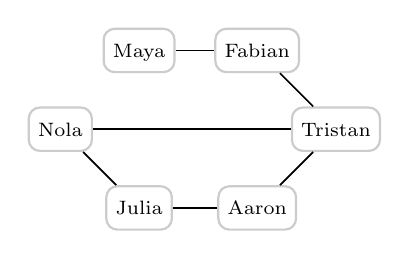
\begin{tikzpicture}
[nodes={text height=.7em, text depth=.2em, draw=black!20, thick, fill=white, font=\scriptsize},
 >=stealth, rounded corners, semithick]
\node (Nola) at (0,0) {Nola};
\node (Maya) at (1,1) {Maya};
\node (Julia) at (1,-1) {Julia};
\node (Fabian) at (2.5,1) {Fabian};
\node (Aaron) at (2.5,-1) {Aaron};
\node (Tristan) at (3.5,0) {Tristan};
\draw (Maya) -- (Fabian);
\draw (Fabian) -- (Tristan);
\draw (Tristan) -- (Aaron);
\draw (Aaron) -- (Julia);
\draw (Julia) -- (Nola);
\draw (Nola) -- (Tristan);
\end{tikzpicture}
%\end{center}
\caption{Example CSP graph: kids and their relationships}
\label{fig:intro-example-graph}
\end{wrapfigure}
Consider a typical \gls{CSP} that deals with the following scenario. Assume you are organizing a holiday camp for kids. Some kids know each other already, some don't. You plan to assign the kids to their dorms in such a way that the kids may become acquainted with other kids they do not yet know. Figure~\vref{fig:intro-example-graph} illustrates the relationships between the kids.

The drawing shows the relationships as a graph, where the children are represented by vertices. The edges between them show the acquaintances, that is, if two kids know each other, there is an edge between them in the graph.

%To be formal, the definition:
%%(see Section~\ref{sec:graphs} for a formal definition of a graph).
%\newglossaryentry{graph}{name=Graph,text=graph,description={\nopostdesc}}
%\newglossaryentry{vertex}{name=vertex,plural=vertices,description={\nopostdesc},parent=graph}
%\newglossaryentry{edge}{name=edge,description={\nopostdesc},parent=graph}
%\begin{Definition}[\gls{graph}]
%A \gls{graph} consists of a set of \glspl{vertex} and a set of \glspl{edge}. Each edge connects two vertices, and is represented as a pair of vertices.
%\end{Definition}

So our plan is to assign the kids to rooms such that no two kids in any room have an edge between them in the graph. In this example, is this possible with two rooms? Indeed, it is: we could give one room to Tristan, Julia and Maya, and another to Nola, Aaron and Fabian.

This is a variant of a problem called Graph Coloring Problem, also known as Chromatic Number, which asks, given a graph, if it is possible to assign $k$ colors to the vertices in the graph, such that each edge only connects vertices that have different colors. In our example, we have asked if this is possible with $k=2$. With more than two colors, the decision version of the Graph Coloring Problem---e.g., is there a k-coloring with $k=3$?---is already significantly harder to solve; in fact, for $k \ge 3$ it is known to be $\NP$-complete (see~\parencite{DBLP:books/daglib/0018514} for an introduction to complexity theory). The optimization version, i.e., computing the chromatic number, is $\NP$-hard as well. To give an idea what this means, consider the example again. Since we have 6 kids and two rooms, there are $2^6 = 64$ possible kids-to-rooms assignments. Despite these $64$ possibilities, we were quick in finding a solution to the example here, so we would expect that it would not be that hard to solve the same problem for, say, a class of 25 pupils. However, when asking whether we can assign the 25 pupils to $k=5$ rooms in the same way, we already face $5^{25} = 2.9802322\cdot 10^{17}$ possible assignments. Assuming that evaluating a single assignment takes a computer one hundredths of a second, testing all possible assignments would still take 94502544 years. This demonstrates the complexity of $\NP$-complete problems, where the runtime grows exponentially with the size of the problem instance.

Fortunately, we might still be able to solve such an instance in a reasonable amount of time, if it has a special structure, as we will see below.

\smallbreak
Typically, the Graph Coloring Problem is formulated as a \gls{CSP}:
\begin{Definition}[\gls{CSP}]
   A \gls{CSP} is a triple $\langle V, D, C \rangle$, where $V = \{v_1, \ldots, v_n\}$ is a set of variables, $D = \{d_1, \ldots, d_n\}$ a set of finite domains (which contain the values that can be assigned to the variables in $V$, respectively), and $C = \{c_1, \ldots, c_m\}$ a set of constraints (each constraint is given as a pair of a set of $k$ variables $\in V$ and a $k$-ary relation that represents the actual constraint on these variables). A solution to a \gls{CSP} is an assignment of values to all variables, such that all constraint relations are fulfilled.
\end{Definition}
In the case of the example above, we could use one variable for each kid ($V = \{\mathrm{Nola}, \mathrm{Tristan}, \ldots\}$), and use the room numbers as domains for these variables (e.g., $\mathrm{Nola} = 2$ means that Nola is assigned to the room 2). The constraints would be formulas that allow two variables to have the same number only if they are not connected with an edge in the underlying graph.

\subsection*{Tree Decomposition and Treewidth}
%           ^^^^^^^^^^^^^^^^^^^^^^^^^^^^^^^^
It turns out that a \gls{CSP} instance is tractable if it features certain structural properties. Either it is tractable due to a restricted structure of the contraint scopes, or due to particular properties of the constraint relations~\parencite{Gottlob2000243,pearson1997survey}. In order to identify and solve tractable \glspl{CSP} instances, decomposition methods may be used. In this work, we focus on \emph{tree decompositions}, and a property called \emph{treewidth}. Creating a tree decomposition of a graph means to translate the original graph into another graph, the tree decomposition, according to a set of rules. The formal definitions of tree decomposition and treewidth are given in Section~\vref{sec:treewidth}.

Interestingly, a small treewidth causes shorter running times: if the underlying graph has bounded treewidth, the problem can be solved in $\mathcal{O}(n \cdot d^{t+1})$, where $n$ is the number of variables, $d$ is the maximal domain size of any variable, and $t$ is the treewidth of the instance~\parencite{Russell:2003:AIM:773294}. Clearly, the treewidth has a great impact on the runtime (as $t$ is in the exponent); therefore the goal is to find a tree decomposition of minimal width, which can then be used to solve the original problem.

Relating to the school class problem: if we can find a tree decomposition of the underlying acquaintance graph with a sufficiently small width, we are able to solve it quickly.

In order to illustrate how tree decompositions may be derived, we consider the first example again, and develop one possible tree decomposition off the original graph. A common way to generate a tree decomposition is by \emph{vertex elimination}, where vertices are removed from the original graph one by one, according to an \emph{elimination ordering}. An elimination ordering then explicitly defines the resulting tree decomposition. To illustrate the elimination process, we use the following elimination ordering with the previous example: Fabian, Julia, Maya, Aaron, Nola, Tristan. Please note that this ordering is completely arbitrary. Most of the algorithms that solve this problem essentially do the same: they calculate the width of tree decompositions using the steps that are illustrated in the following example, according to (intelligently) guessed elimination orderings. The aim of the algorithms is to be good at finding these orderings, so that the width of the resulting tree decomposition is as small as possible.

We start by eliminating the first vertex: Fabian. When removing a vertex from the original graph (on the left), we create a tree node in the tree decomposition (on the right) that contains the eliminated vertex and all its neighbors. When removing Fabian, we create a node that contains Fabian, Maya and Tristan:
\begin{tightcenter}
%\begin{verbatim}
%       Maya ---- FABIAN ----            -= F,M,T =-
%                            \                      
%Nola -------------------- Tristan                  
%  \                         /                      
%   --- Julia --- Aaron -----                       
%\end{verbatim}
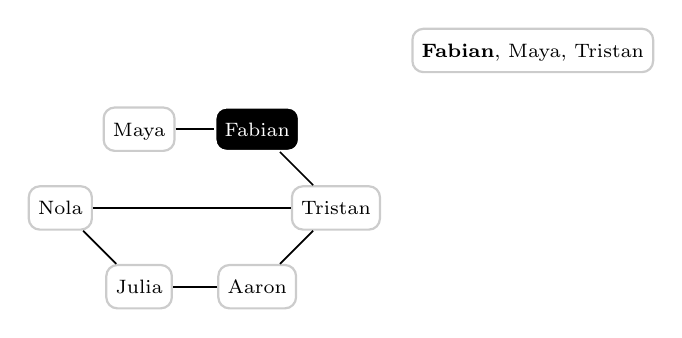
\begin{tikzpicture}
[nodes={text height=.7em, text depth=.2em, draw=black!20, thick, fill=white, font=\scriptsize},
 >=stealth, rounded corners, semithick]
\node (Nola) at (0,0) {Nola};
\node (Maya) at (1,1) {Maya};
\node (Julia) at (1,-1) {Julia};
\node (Fabian) at (2.5,1) [color=white, fill=black] {Fabian};
\node (Aaron) at (2.5,-1) {Aaron};
\node (Tristan) at (3.5,0) {Tristan};
\draw (Maya) -- (Fabian);
\draw (Fabian) -- (Tristan);
\draw (Tristan) -- (Aaron);
\draw (Aaron) -- (Julia);
\draw (Julia) -- (Nola);
\draw (Nola) -- (Tristan);

\node (FMT) at (6,2) {\textbf{Fabian}, Maya, Tristan};
\end{tikzpicture}
\end{tightcenter}
After removing a vertex, we connect in the original graph all its previous neighbors with each other. In the case of Fabian, we connect Maya and Tristan. Then we remove the next vertex: Julia.
\begin{tightcenter}
%\begin{verbatim}
%       Maya ----------------            -= F,M,T =-
%                            \                         -= J,N,A =-
%Nola -------------------- Tristan                  
%  \                         /                      
%   --- JULIA --- Aaron -----                       
%\end{verbatim}
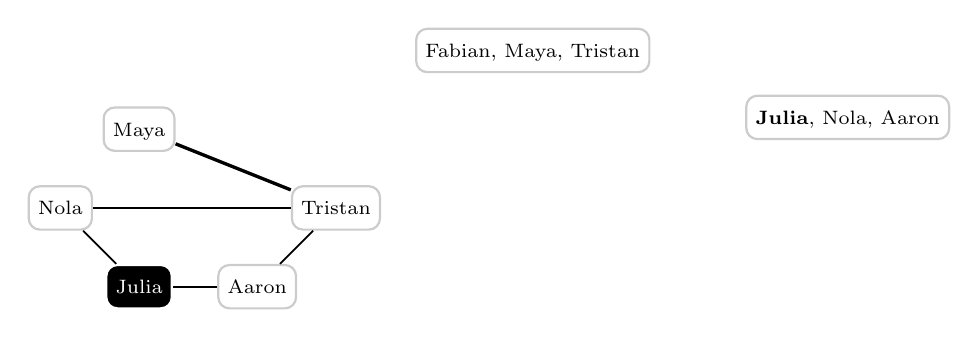
\begin{tikzpicture}
[nodes={text height=.7em, text depth=.2em, draw=black!20, thick, fill=white, font=\scriptsize},
 >=stealth, rounded corners, semithick]
\node (Nola) at (0,0) {Nola};
\node (Maya) at (1,1) {Maya};
\node (Julia) at (1,-1) [color=white, fill=black] {Julia};
\node (Aaron) at (2.5,-1) {Aaron};
\node (Tristan) at (3.5,0) {Tristan};
\draw [very thick] (Maya) -- (Tristan);
\draw (Tristan) -- (Aaron);
\draw (Aaron) -- (Julia);
\draw (Julia) -- (Nola);
\draw (Nola) -- (Tristan);

\node (FMT) at (6,2) {Fabian, Maya, Tristan};
\node (JNA) at (10,1.15) {\textbf{Julia}, Nola, Aaron};
\end{tikzpicture}
\end{tightcenter}
A node in the tree decomposition should be connected to the \emph{next} node that is created because of the elimination of a vertex that occurs in it. In this case, Julia does not appear in the first node, so the two nodes are not connected. We continue with Maya.
\begin{tightcenter}
%\begin{verbatim}
%       MAYA ----------------            -= F,M,T =-
%                            \                 |       -= J,N,A =-
%Nola -------------------- Tristan         -= M,T =-
%  \                         /                      
%   ------------- Aaron -----                       
%\end{verbatim}
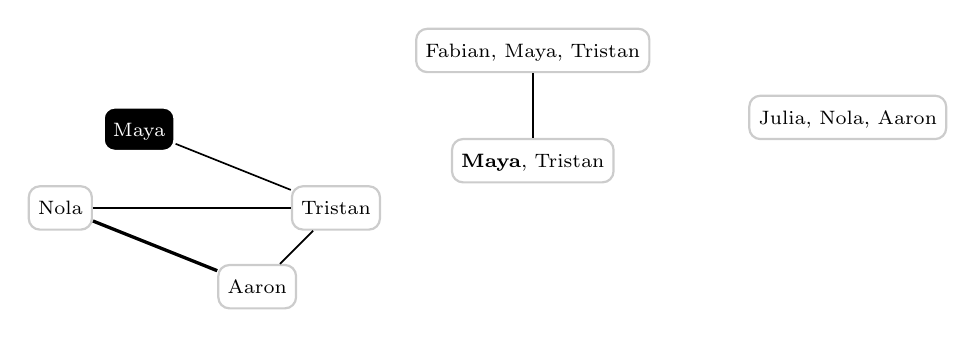
\begin{tikzpicture}
[nodes={text height=.7em, text depth=.2em, draw=black!20, thick, fill=white, font=\scriptsize},
 >=stealth, rounded corners, semithick]
\node (Nola) at (0,0) {Nola};
\node (Maya) at (1,1) [color=white, fill=black] {Maya};
\node (Aaron) at (2.5,-1) {Aaron};
\node (Tristan) at (3.5,0) {Tristan};
\draw (Maya) -- (Tristan);
\draw (Tristan) -- (Aaron);
\draw [very thick] (Aaron) -- (Nola);
\draw (Nola) -- (Tristan);

\node (FMT) at (6,2) {Fabian, Maya, Tristan};
\node (JNA) at (10,1.15) {Julia, Nola, Aaron};
\node (MT) at (6,.6) {\textbf{Maya}, Tristan};
\draw (FMT) -- (MT);
\end{tikzpicture}
\end{tightcenter}
Since Maya is contained in the first node, and the first node has not been connected to a newer node yet, we connect the two nodes.  Next: Aaron.
\begin{tightcenter}
%\begin{verbatim}
%                                        -= F,M,T =-
%                                              |       -= J,N,A =-
%Nola -------------------- Tristan         -= M,T =-        |
%  \                         /                              |
%   ------------- AARON -----                          -= A,N,T =-
%\end{verbatim}
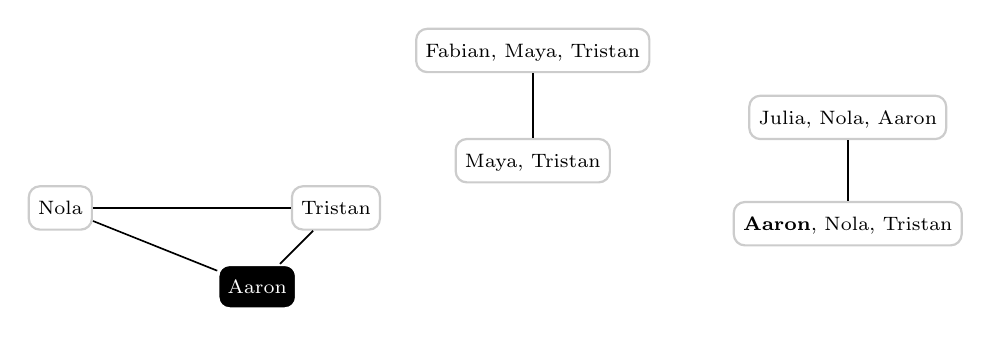
\begin{tikzpicture}
[nodes={text height=.7em, text depth=.2em, draw=black!20, thick, fill=white, font=\scriptsize},
 >=stealth, rounded corners, semithick]
\node (Nola) at (0,0) {Nola};
\node (Aaron) at (2.5,-1) [color=white, fill=black] {Aaron};
\node (Tristan) at (3.5,0) {Tristan};
\draw (Tristan) -- (Aaron);
\draw (Aaron) -- (Nola);
\draw (Nola) -- (Tristan);

\node (FMT) at (6,2) {Fabian, Maya, Tristan};
\node (JNA) at (10,1.15) {Julia, Nola, Aaron};
\node (MT) at (6,.6) {Maya, Tristan};
\node (ANT) at (10,-0.2) {\textbf{Aaron}, Nola, Tristan};
\draw (FMT) -- (MT);
\draw (JNA) -- (ANT);
\end{tikzpicture}
\end{tightcenter}
Aaron's tree node too gets connected to a previous node. The two remaining vertices are Nola and Tristan.
\begin{tightcenter}
%\begin{verbatim}
%                                        -= F,M,T =-
%                                              |       -= J,N,A =-
%NOLA -------------------- Tristan         -= M,T =-        |
%                                                           |
%                                                      -= A,N,T =-
%                                                           |      
%                                                       -= N,T =-
%\end{verbatim}
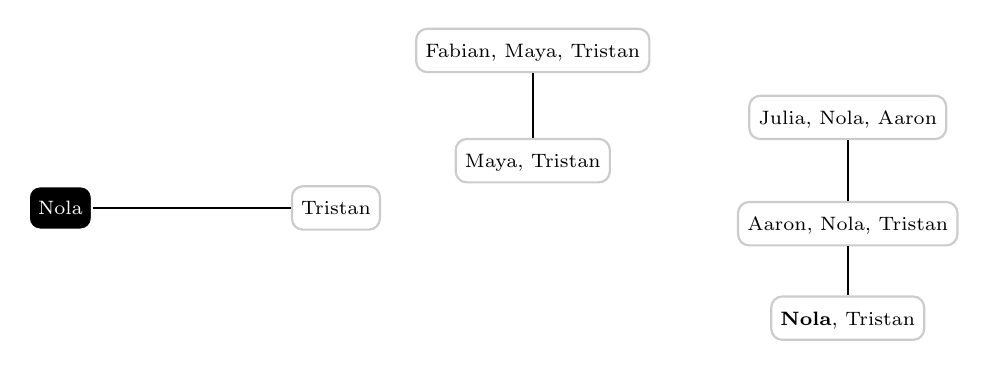
\begin{tikzpicture}
[nodes={text height=.7em, text depth=.2em, draw=black!20, thick, fill=white, font=\scriptsize},
 >=stealth, rounded corners, semithick]
\node (Nola) at (0,0) [color=white, fill=black] {Nola};
\node (Tristan) at (3.5,0) {Tristan};
\draw (Nola) -- (Tristan);

\node (FMT) at (6,2) {Fabian, Maya, Tristan};
\node (JNA) at (10,1.15) {Julia, Nola, Aaron};
\node (MT) at (6,.6) {Maya, Tristan};
\node (ANT) at (10,-0.2) {Aaron, Nola, Tristan};
\node (NT) at (10,-1.4) {\textbf{Nola}, Tristan};
\draw (FMT) -- (MT);
\draw (JNA) -- (ANT) -- (NT);
\end{tikzpicture}
\end{tightcenter}

\begin{tightcenter}
%\begin{verbatim}
%                                        -= F,M,T =-
%                                              |       -= J,N,A =-
%                          TRISTAN         -= M,T =-        |
%                                              |            |
%                                              |       -= A,N,T =-
%                                              |            |      
%                                               \       -= N,T =-
%                                                \         /
%                                                 \-= T =-/
%\end{verbatim}
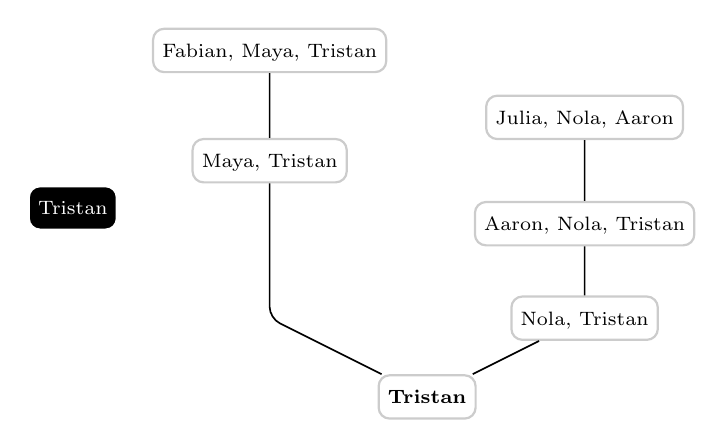
\begin{tikzpicture}
[nodes={text height=.7em, text depth=.2em, draw=black!20, thick, fill=white, font=\scriptsize},
 >=stealth, rounded corners, semithick]
\node (Tristan) at (3.5,0) [color=white, fill=black] {Tristan};

\node (FMT) at (6,2) {Fabian, Maya, Tristan};
\node (JNA) at (10,1.15) {Julia, Nola, Aaron};
\node (MT) at (6,.6) {Maya, Tristan};
\node (ANT) at (10,-0.2) {Aaron, Nola, Tristan};
\node (NT) at (10,-1.4) {Nola, Tristan};
\node (T) at (8,-2.4) {\textbf{Tristan}};
\draw (FMT) -- (MT) -- (6,-1.4) -- (T);
\draw (JNA) -- (ANT) -- (NT) -- (T);
\end{tikzpicture}
\end{tightcenter}
Tristan is present in two nodes, which both have not been connected to any newer nodes yet, so Tristan's node gets connected to both.

Finally, we may delete all nodes where the vertices are fully contained in a neighbor node:
\begin{center}
%\begin{verbatim}
%-= F,M,T =-                     -= F,M,T =-              
%      |       -= J,N,A =-             |       -= J,N,A =-
%  -= M,T =-        |                  |            |     
%      |            |                  |            |     
%      +--= A,N,T =-+                  +--= A,N,T =-+    
%             |             =>                           
%         -= N,T =-                                      
%             |                                          
%          -= T =-                                       
%\end{verbatim}
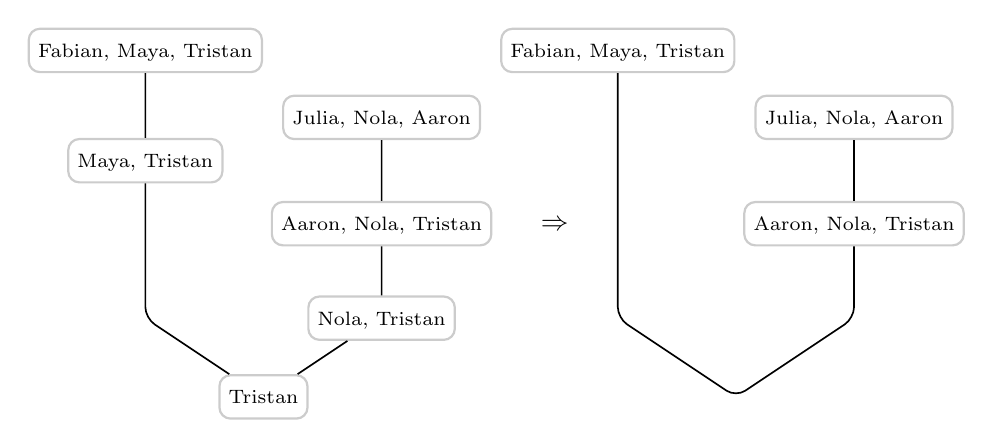
\begin{tikzpicture}
[nodes={text height=.7em, text depth=.2em, draw=black!20, thick, fill=white, font=\scriptsize},
 >=stealth, rounded corners, semithick]
\node (FMT) at (0,2) {Fabian, Maya, Tristan};
\node (JNA) at (3,1.15) {Julia, Nola, Aaron};
\node (MT) at (0,.6) {Maya, Tristan};
\node (ANT) at (3,-0.2) {Aaron, Nola, Tristan};
\node (NT) at (3,-1.4) {Nola, Tristan};
\node (T) at (1.5,-2.4) {Tristan};
\draw (FMT) -- (MT) -- (0,-1.4) -- (T);
\draw (JNA) -- (ANT) -- (NT) -- (T);

\node at (5.2,-.2) [draw=none,font=\normalsize] {$\Rightarrow$};

\node (XFMT) at (6,2) {Fabian, Maya, Tristan};
\node (XJNA) at (9,1.15) {Julia, Nola, Aaron};
\node (XANT) at (9,-0.2) {Aaron, Nola, Tristan};
\draw (XFMT) -- (6,-1.4) -- (7.5,-2.4) -- (9,-1.4) -- (XANT);
\draw (XJNA) -- (XANT);
\end{tikzpicture}
\end{center}

The intuition behind this tree decomposition is that the nodes represent \emph{subproblems}, and relating subproblems are connected to each other. In this example, we can observe that assigning a room to Tristan influences the possible solutions for the Aaron-Nola-Tristan node; similarly, the assignment for the latter affects the Julia-Nola-Aaron node. The idea is to divide the problem into smaller subproblems, and by concentrating on the subproblems, solve the original problem more efficiently.

%As noted in Definition~\ref{def:treewidth}, the treewidth is defined as the maximal number of vertices in any such node, minus 1; so the treewidth of the tree decomposition we have just created is 2.

%The \emph{treewidth of a graph} is the minimal treewidth of all possible tree decompositions.
Unfortunately, just as solving the original problem, finding the treewidth of a graph (i.e., the minimal width over all tree decompositions; see Definition~\ref{def:tree decomposition}) is $\NP$-hard as well~\parencite{arnborg-1987-complexity}. Consequently, the purpose of the optimization heuristics that are presented in this thesis is to find good upper bounds on the treewidth of given graphs.


\section{Research Questions of This Work}
%        ^^^^^^^^^^^^^^^^^^^^^^^^^^^^^^^
   \label{sec:Research Question}
%
There are different approaches for finding good upper bounds on the treewidths of graphs, as will be discussed in Chapter~\ref{ch:Related Work}. To the best of our knowledge, however, memetic algorithms, which have been applied successfully to other problems in the past, have not yet been applied to this problem. 

\medbreak\noindent%
This work's objectives are:
\begin{itemize}
\item The development of new memetic algorithms for minimizing upper bounds on the treewidth of graphs.
\item An evaluation of the developed memetic algorithms on benchmark instances from the literature and the comparison with state-of-the-art algorithms for tree decompositions.
\end{itemize}

%In this work, three such memetic algorithms are developed, so as to answer the main research question of this thesis:
%\begin{quote}
   %Do heuristics that are based on a \glsdesc{MA}, build as a combination of the metaheuristics \glsdesc{GA} and \glsdesc{ILS}, outperform the incarnation of the individual metaheuristics for the problem at hand, namely \glsfirst{GA-tw}~\parencite{schafhauser-thesis,schafhauser-paper}, representing \glsdesc{GA}s, and \glsfirst{IHA}~\parencite{musliu-2008-ILS}, respresenting \glsdesc{ILS}?
%\end{quote}

%Or in other words: Is it a good idea to combine a \glsdesc{GA} based heuristic with an \glsdesc{ILS} based heuristic, when computing minimal treewidth upper bounds?


%\section{Methodology}
%%        ^^^^^^^^^^^
   %\label{sec:Methodology}
%%
%First, existing literature has been reviewed. Memetic algorithms and general hybrid algorithms, and their application to other problems, have been studied. Then three memetic algorithms, MA1, MA2, and MA3, have been designed, using ideas from~\parencite{moscato-1989,musliu-schafhauser-2007-GA,hammerl-musliu-schafhauser-metaheuristicAlgorithms,musliu-2008-ILS,schafhauser-thesis,schafhauser-paper,widl-thesis,widl-paper}. They have been implemented in \Cpp. Their operational parameters have been determined using parameter tuning software, applied to a set of training instances. Their performance has been evaluated using a second, distinct set of validation instances.


\section{Main Results}
%        ^^^^^^^^^^^^
   \label{sec:Main Results}
%
The main contributions of this work are:
\begin{itemize}
   \item We propose three memetic algorithms for tree decomposition: \gls{MA1}, \gls{MA2} and \gls{MA3}. \gls{MA1} organizes a population of solutions in a randomly initialized ring structure, which is used for employing selection and recombination among the individual solutions according to their vicinity. Each generation is collectively improved using iterated local search. \gls{MA2} is a hybrid between a genetic algorithm that uses elitism for selection, and iterated local search, which is used to improve the best individuals of every generation. Finally, \gls{MA3} implements an existing genetic algorithm design and also incorporates iterated local search, which is applied to a random fraction of each generation. Their parameters have been tuned using state-of-the-art parameter tuning software, and the correlation between those parameters and the corresponding solution quality has been studied.

\item Our algorithms have been compared with state-of-the-art solvers for tree decomposition. The memetic algorithms cannot outperform them, but they prove to be competitive as they perform equivalently on many benchmark instances.
   One of our algorithms (\gls{MA3}) is able to improve 8 best known upper bounds for instances of the Second \gls{DIMACS} Implementation Challenge~\parencite{dimacs-challenges}.

\item Public open-source implementations have been written from scratch and released under GPLv3. Code quality is ensured by providing high test coverage.
\end{itemize}


\section{Further Organization}
%        ^^^^^^^^^^^^^^^^^^^^
   \label{sec:Further Organization}
%
   In the following, Chapter~\ref{ch:Related Work} discusses the related work. Then Chapter~\ref{ch:algorithms} introduces our memetic algorithms. Chapter~\ref{ch:eval1} elaborates on parameter tuning, and also inspects possible parameter correlations. In Chapter~\ref{ch:Results} the experimental evaluation of the memetic algorithms is presented. Finally, Chapter~\ref{ch:Conclusions} gives a conclusion.
   
   Additionally, Appendix~\ref{appendix:boring-validation-instances} list results from the algorithm validation that have been omitted in Section~\ref{ch:Results} for brevity.


%\noindent\rule{\textwidth}{2pt}
%\noindent\rule{\textwidth}{2pt}
%\textbf{Narrative Flow:}\\
%\textbf{Introduction:} Different classes of problems (probably); here is a nice NP hard problem; it turns out there is another way to solve it: tree decomposition. What is tree decomposition? It only helps if the decomposition has a small treewidth. So this is why computing a decomposition with minimal treewidth helps to solve the original problem. There are many interesting NP hard problems, where this technique could allow us to solve them faster. There are methods already, but it would be great to improve on the existing upper bounds. Contributions! \textbf{The Problem:} Treewidth of graph can be computed like this and like that. In most publications this is used. This works like this, because of this. \textbf{My Idea:} Here is my idea: hybridization could be the key. \textbf{The Details:} Methodology and stuff: what and how. Implementation details. Parameter tuning. Results. My idea works: better results. \textbf{Related Work:} Other approaches are worse or almost as good and can be found there and there. \textbf{Conclusions and further work:} ....
%\begin{enumerate}
   %\item Introduction\\
      %\textit{in which we elaborate on tree decomposition, treewidth, and on why this is interesting for concrete applications}
%\end{enumerate}
%\noindent\rule{\textwidth}{.5pt}
%\begin{itemize}
    %\item What is a problem, what an instance
    %\item How to represent in instance using a graph
    %\item What is a tree decomposition
    %\item Why are we interested in a TD?
    %\begin{itemize} \item     Applications \end{itemize}
    %\item How it is computed today
    %\item Is the combination of two particular algorithms beneficial for solving the described problem? Or more specifically: does hybridization of GA and ILS improve on the individual performance in the case of treewidth minimization?
%\end{itemize}
%\noindent\rule{\textwidth}{2pt}
%\pfbreak

%\noindent\rule{\textwidth}{2pt}
%-> applications
%Treewidth and Pure Nash Equilibria
%Antonis Thomas and Jan van Leeuwen

%\noindent\rule[.8\baselineskip]{\textwidth}{2pt}

%In the 70ies of the last century, scientists introduced \emph{\NP-completeness}, a class for problems with solutions that can be verified quickly (in polynomial time), but require exponential time (in the size of the instance) to be found.\footnote{Formally, a problem is \NP-complete if it can be solved by a nondeterministic turing machine in polynomial time, and there exists a polynomial-time reduction that reduces a known \NP-complete problem to it.} Even today, the question whether this class exists at all is still unsolved (the famous \enquote{\P\ versus \NP} question). Despite this uncertainty, many interesting problems have been proofed to be \NP-complete. As an example, consider the following map of\todo{schaut zwar cool aus, aber a simplere karte aus der ma leichter a CSP beispiel machen kann wär vlt sinnvoller} Europe:
%\begin{center}
   %\includegraphics[width=0.5\textwidth,keepaspectratio]{./img/EuropeColorMap.jpg}
%\end{center}
%\newglossaryentry{GCP}{name=Graph Coloring Problem,description={\nopostdesc}}
%Suppose\Index{\gls{GCP}} you would want every two adjacent countries to have different colors. Could you do this with 2 colors only? Or with 3? Or would you need 4? Even though this does not look like a difficult question at first, it turns out that when the number of colors is larger than 2, the problem is already \NP-complete. In literature, this problem is called the Graph Coloring Problem\footnote{Also known as \emph{Chromatic Number}, as listed in Karp's 21 \NP-Complete Problems. See \url{http://en.wikipedia.org/wiki/Graph_coloring} for more information.}.

%The Graph Coloring Problem can be modelled as a \Index{\glsentrydesc{CSP}}\gls{CSP}; a mathematical problem defined in terms of variables, domains, and constraint relations between those variables subject to those domains\footnote{See \url{http://en.wikipedia.org/wiki/Constraint_satisfaction_problem} for further reading.}. The great feature of \glspl{CSP} is that many interesting \NP-hard problems can be formulated as such a problem, which means that being able to solve \glspl{CSP} quickly means being able to solve all those interesting problems quickly as well. But first, we ought to know what a \gls{CSP} generally looks like. A formal definition:
%\begin{Definition}[\gls{CSP}]
   %A \gls{CSP} is a triple $\langle V, D, C \rangle$, where $V = \{v_1, \ldots, v_n\}$ is a set of variables, $D = \{d_1, \ldots, d_n\}$ a set of finite domains (which contain the values that can be assigned to the variables in $V$, respectively), and $C = \{c_1, \ldots, c_m\}$ a set of constraints (each constraint is given as a pair of a set of $k$ variables $\in V$ and a $k$-ary relation that represents the actual constraint on these variables). A solution to a \gls{CSP} is \emph{complete} -- i.e., the solution assigns a value $\in d_i$ to each $v_i \in V$ -- and \emph{consistent}, which means that it satisfies all constraint relations in $C$.
%\end{Definition}

%The example displayed above can be represented as a simple graph, as shown in Figure~\vref{fig:europe-graph}\todo{mit aner (evtl anderen) karten a CSP beispiel basteln}. The \gls{CSP}\todo{formulate CSP} formulation:
%\begin{align*}
   %\text{Variables}~V &= \{\text{holy roman empire}, \ldots\}\\
   %\text{Domains}~D &= \{\{\text{green, yellow, blue, \ldots}\}, \{\text{green, yellow, blue, \ldots}\}, \ldots\}\\
   %\text{Constraints}~C &= \text{no two neighboring countries may be colored the same}
%\end{align*}

%%In the 80ies, it became apparent that many \NP-complete problems can be solved efficiently by dynamic programming when their instances have bounded \emph{treewidth}, a feature related to the \emph{tree decomposition} of a graph.
%So we have established that a \gls{CSP} may be represented as a Graph\todo{Hypergraph, actually}. Instead of directly using this graph to solve the problem, however, we \emph{decompose} it into a tree-like structure. The details of this so-called tree\Index{\gls{tdecomp}} decomposition are described in the next chapter; for now, let's assume that it is some kind of transformation that translates a graph into another, different graph. For instance, tree decomposition can be used to transform a graph that represents a \gls{CSP} to another graph, that looks differently, but still represents the same problem instance. The motivation for doing this is that with the right decomposition, finding a solution to the problem may be easier than with the original graph. In fact, if a feature of the tree decomposition called \emph{treewidth}\Index{\gls{tw}} is minimal (or small) for a given instance, a problem that is known to be intractable becomes tractable in the case of this instance, when the solving algorithm operates on this minimal-width tree decomposition.

%\emph{That is why finding tree decompositions of minimal width is interesting.}

%Today we know that by translating instance graphs to tree decompositions of small treewidth, certain instances of \NP-complete problems can even be solved in linear time (for instance, using dynamic programming approaches). The question that needs to be answered in order to leverage this is:
%\begin{center}
   %\emph{Can we build a tree decomposition of an input graph\\
   %with treewidth of at most $k$?}
%\end{center}
%As expected, this problem is, unfortunately, \NP-complete as well.

%\pfbreak
%\TODO{solving NP problems with metaheuristics. idea that hybridization could bring about improvements.}

%In this thesis the following contributions are presented:
%\begin{itemize}
 %\item The main contribution of this work is answering whether hybridization of two well known and widely used metaheuristics (\glsentryname{GA} and \glsentryname{ILS}) improves on the results of the individual algorithms in the case of treewidth minimization of simple-graph \gls{CSP} instances. Four hybridization variants are put to the test, tuned by an automatic parameter tuner.
 %\item \TODO{more?}
%\end{itemize}
%%\begin{itemize}
   %%\item The main contribution of this work is researching the potential of hybrid approaches to the treewidth decision problem. Two different combinations are introduced in Chapter~\vref{ch:My Idea} and examined in detail in Chapter~\vref{ch:The Details}.
      %%Parameter tuning software has been used to explore whether the presented hybrid algorithms are able to perform equally well over different instances. The tuning process is described in Section~\vref{sec:Parameter Tuning}.
   %%\item For selected instances of the widely used DIMACS graph coloring benchmarks, existing upper bounds on treewidth are tested and improved (Chapter~\vref{ch:The Details}). The results are related to previous work in Chapters~\vref{ch:The Details} and~\vref{ch:Related Work}.
%%\end{itemize}

%\bigskip
%\scalebox{2}{\textbf{Put (some of) this stuff into}}
%\scalebox{2}{\textbf{Chap 2 Preliminaries}}
%\bigskip

%\section{The Problem}
%\label{The Problem}

%Before discussing ways to find the minimal-treewidth tree decomposition, the latter are introduced, starting with an example. In introduction contains an example for a \NP-complete problem, namely the graph coloring problem. In order to understand what a tree decomposition is, we consider an exemplary instance to this problem:
%%
%\begin{center}
   %\begin{tikzpicture}
      %[scale=0.65,
      %vertex/.style={circle,draw=blue!50,fill=blue!20,thick}]
      %\node[vertex] (1) at (2,2) {1};
      %\node[vertex] (2) at (2,0) {2};
      %\node[vertex] (3) at (4,1) {3};
      %\node[vertex] (4) at (6,0) {4};
      %\node[vertex] (5) at (6,2) {5};
      %\node[vertex] (6) at (8,1) {6};
      %\node[vertex] (7) at (0,1) {7};
      %\draw (1) to [out=270,in= 90] (2);
      %\draw (1) to [out=  0,in=100] (3);
      %\draw (1) to [out=180,in= 80] (7);
      %\draw (2) to [out=180,in=280] (7);
      %\draw (2) to [out=  0,in=260] (3);
      %\draw (3) to [out=280,in=180] (4);
      %\draw (3) to [out= 80,in=180] (5);
      %\draw (4) to [out= 90,in=270] (5);
      %\draw (4) to [out=  0,in=260] (6);
      %\draw (5) to [out=  0,in=100] (6);
   %\end{tikzpicture}
%\end{center}
%%
%This time, we consider \emph{vertices} instead of countries to color, and instead of borders between them, we see \emph{edges}. Intuitively, a tree decomposition is a way to map this graph into a tree, where adjacent vertices intersect in the vertices of subtrees of this tree. While the exact definition follows afterwards, tree decomposition is best understood using an illustration. Figure~\vref{fig:minTestFill decomposition} shows a possible tree decomposition of the example shown above, visualizing the computational steps. The treewidth for this example is 4; it is defined as the maximum of the number of vertices of any node of the tree decomposition, minus one (see Definition~\vref{def:treewidth}).

%%\begin{figure}
   %%\centering
   %%\usetikzlibrary{arrows.meta,backgrounds,fit}
\begin{tikzpicture}
[scale=0.65,
 show background rectangle, inner frame sep=2.5em,
 background rectangle/.style={},
 vertex/.style={circle,draw=blue!50,fill=blue!20,thick},
 selectedvertex/.style={circle,draw=red!50,fill=red!20,thick},
 nextvertex/.style={circle,draw=blue!50,fill=violet!30,thick},
 edge/.style={thick},
 newedge/.style={dashed,thick},
 treenode/.style={rectangle,rounded corners=4,inner sep=6,draw=black,fill=gray!10,thick},
 treeedge/.style={very thick},
 hint/.style={-{Latex[]},very thin}]
\node[rectangle,draw=black!30,rounded corners=4,inner sep=6] at (6,4.8) {Elimination Ordering: 3 -- 5 -- 2 -- 6 -- 7 -- 4 -- 1};

\node[        vertex] (1) at (2,2) {1};
\node[        vertex] (2) at (2,0) {2};
\node[selectedvertex] (3) at (4,1) {3};
\node[        vertex] (4) at (6,0) {4};
\node[        vertex] (5) at (6,2) {5};
\node[        vertex] (6) at (8,1) {6};
\node[        vertex] (7) at (0,1) {7};
\draw[   edge] (1) to [out=270,in= 90] (2);
\draw[   edge] (1) to [out=  0,in=100] (3);
\draw[   edge] (1) to [out=180,in= 80] (7);
\draw[   edge] (2) to [out=180,in=280] (7);
\draw[   edge] (2) to [out=  0,in=260] (3);
\draw[   edge] (3) to [out=280,in=180] (4);
\draw[   edge] (3) to [out= 80,in=180] (5);
\draw[   edge] (4) to [out= 90,in=270] (5);
\draw[   edge] (4) to [out=  0,in=260] (6);
\draw[   edge] (5) to [out=  0,in=100] (6);

\node[        vertex] (a1) at (2,-2) {1};
\node[        vertex] (a2) at (2,-4) {2};
\node[        vertex] (a4) at (6,-4) {4};
\node[selectedvertex] (a5) at (6,-2) {5};
\node[        vertex] (a6) at (8,-3) {6};
\node[        vertex] (a7) at (0,-3) {7};
\draw[   edge] (a1) to [out=270,in= 90] (a2);
\draw[newedge] (a1) to [out= 10,in=170] (a5);
\draw[newedge] (a1) to [out=  0,in=180] (a4);
\draw[   edge] (a1) to [out=180,in= 80] (a7);
\draw[   edge] (a2) to [out=180,in=280] (a7);
\draw[newedge] (a2) to [out=350,in=190] (a4);
\draw[newedge] (a2) to [out=  0,in=180] (a5);
\draw[   edge] (a4) to [out= 90,in=270] (a5);
\draw[   edge] (a4) to [out=  0,in=260] (a6);
\draw[   edge] (a5) to [out=  0,in=100] (a6);

\node[        vertex] (b1) at (2,-6) {1};
\node[selectedvertex] (b2) at (2,-8) {2};
\node[        vertex] (b4) at (6,-8) {4};
\node[        vertex] (b6) at (8,-7) {6};
\node[        vertex] (b7) at (0,-7) {7};
\draw[   edge] (b1) to [out=270,in= 90] (b2);
\draw[   edge] (b1) to [out=  0,in=180] (b4);
\draw[newedge] (b1) to [out=  0,in=150] (b6);
\draw[   edge] (b1) to [out=180,in= 80] (b7);
\draw[   edge] (b2) to [out=180,in=280] (b7);
\draw[   edge] (b2) to [out=350,in=190] (b4);
\draw[newedge] (b2) to [out=  0,in=180] (b6);
\draw[   edge] (b4) to [out=  0,in=260] (b6);

\node[        vertex] (c1) at (2,-10) {1};
\node[        vertex] (c4) at (6,-12) {4};
\node[selectedvertex] (c6) at (8,-11) {6};
\node[        vertex] (c7) at (0,-11) {7};
\draw[   edge] (c1) to [out=  0,in=150] (c6);
\draw[   edge] (c1) to [out=  0,in=180] (c4);
\draw[   edge] (c1) to [out=180,in= 80] (c7);
\draw[   edge] (c4) to [out=  0,in=260] (c6);
\draw[newedge] (c4) to [out=200,in=320] (c7);
\draw[newedge] (c6) to [out=178,in=  2] (c7);

\node[        vertex] (d1) at (2,-14) {1};
\node[        vertex] (d4) at (6,-16) {4};
\node[selectedvertex] (d7) at (0,-15) {7};
\draw[   edge] (d1) to [out=  0,in=180] (d4);
\draw[   edge] (d1) to [out=180,in= 80] (d7);
\draw[   edge] (d4) to [out=200,in=320] (d7);

\node[        vertex] (e1) at (2,-18) {1};
\node[selectedvertex] (e4) at (6,-20) {4};
\draw[   edge] (e1) to [out=0,in=180] (e4);

\node[treenode] (A) at (12,1) {3, 5, 2, 4, 1};
\draw[hint] (4,1.5) .. controls (4.3,4) and (10,4) .. (11,1.5);
\node[treenode] (B) at (12,-3) {5, 2, 6, 4, 1};
\draw[hint] (6.2,-1.6) .. controls (8,-0.5) and (10.5,-1) .. (11,-2.5);
\draw[treeedge] (A) to (B);
\node[treenode] (C) at (12,-7) {2, 6, 7, 4, 1};
\draw[hint] (2.3,-7.6) .. controls (4,-5.2) and (10.6,-5.2) .. (11,-6.5);
\draw[treeedge] (B) to (C);
\node[treenode] (D) at (12,-11) {6, 7, 4, 1};
\draw[hint] (8.1,-10.6) .. controls (8.6,-9.2) and (10.8,-9.2) .. (11.2,-10.5);
\draw[treeedge] (C) to (D);
\node[treenode] (E) at (12,-15) {7, 4, 1};
\draw[hint] (0.5,-15) .. controls (7,-17) and (10,-11.5) .. (11.4,-14.5);
\draw[treeedge] (D) to (E);
\node[treenode] (F) at (12,-19) {4, 1};
\draw[hint] (6.2,-19.5) .. controls (7.3,-17.3) and (11.3,-17) .. (11.7,-18.5);
\draw[treeedge] (E) to (F);


\end{tikzpicture}

   %%\caption{TODO}
   %%\label{fig:minTestFill decomposition}
%%\end{figure}

%While there are different ways to compute a tree decomposition, the most common one is \emph{vertex elimination}, which is also shown in Figure~\vref{fig:minTestFill decomposition}. Vertex elimination works by removing vertices from the orignal graph (those colored in red) after some \emph{elimination ordering}, after connecting all remaining neighbors of this node with the one neighbor that comes first in the elimination ordering and has not been removed yet (those colored in green). This way, we build a triangulated graph at every step, and can perceive the size of the largest clique\footnote{A \emph{clique} is a maximal complete subgraph, where \emph{complete subgraph} means that all vertices that belong to that subgraph are connected to each other.} during the vertex elimination as the treewidth of the resulting tree decomposition.

%\section{Formal Definitions}
%This section gives the formal definitions of tree decomposition and treewidth, which are used throughout this thesis, taken from~\parencite{bodlaender-1998-perfectEliminationOrdering}.

   %\begin{Definition}[Tree Decomposition]\label{def:tree decomposition}
      %A tree decomposition of a graph $G=(V,E)$ is a pair $(\{X_i \;|\; i \in I\},\,T=(I,F))$ with $\{X_i \;|\; i \in I\}$ a family of subsets of $V$, one for each node of $T$, and $T$ a tree such that
      %\begin{itemize}
         %\item $\bigcup_{i \in I} X_i = V$
         %\item For all edges $(v,w) \in E$, there exists an $i \in I$ with $v \in X_i$ and $w \in X_i$.
         %\item For all $i,j,k \in I$: if $j$ is on the path from $i$ to $k$ in $T$, then $X_i \cap X_k \subseteq X_j$. (This is equivalent to: For all $v \in V$, the set of nodes $\{i \in I \;|\; v \in X_i\}$ forms a connected part, i.e., a subtree, of $T$.)
      %\end{itemize}
   %\end{Definition}

   %\begin{Definition}[Treewidth]\label{def:treewidth}
      %The width of a tree decomposition $(\{X_i \;|\; i \in I\},\,T=(I,F))$ is $\max_{i \in I} \abs{X_i} - 1$. The treewidth of a graph $G$ is the minimum width over all possible tree decompositions of $G$.
   %\end{Definition}

%\section{Minimal-Width Tree Decomposition}
   %As decribed above, vertex elimination is a tool for finding tree decompositions of a given graph. A vertex elimination is characterized by its elimination ordering, which is just the order in which the vertices get removed from the original graph during the triangulation process.

   %The algorithms presented in this thesis strive to compute good upper bounds on the treewidth of any given input graph. Using vertex elimination, the goal translates to trying to find the \emph{perfect elimination ordering} for vertex elimination, that is, the ordering that, when given to the vertex elimination algorithm, creates a tree decomposition of minimal width.

%\TODO{how and why does vertex elimination exactly work? + references}



%\section{Hybrid Algorithms for Tree Decomposition}
%\label{My Idea}

%In the past, many different algorithms have been designed to compute good upper bounds on the treewidth of arbitraty input graphs (they are listed and discussed in Chapter~\vref{ch:Related Work}). The idea behind this work is to create hybrid algorithms by combining two heuristic techniques that individually have been applied to the problem already, and compare the results in order to assess the value of the hybridization. The reasoning behind the hybridization is that often heuristics perform good on some instances, but worse on other. Intuitively, combining two different heuristics should enable the resulting algorithm to perform equally well over the majority of possible input instances.

%Previous experiments in other problem domains have shown hybrid approaches to be effective, for instance with the break scheduling problem~\parencite{widl-2010-breakscheduling} or the vehicle routing problem~\parencite{shaw-2000-solvingVrpUsingCspAndMetaheuristics}.

%\section{A Memetic Algorithm}
%For the first algorithm, we will combine a \gls{GA} with \gls{ILS}. In literature, this combination is commonly known as \emph{memetic algorithm}\footnote{In the strict sense of a memetic algorithm after Moscato~\parencite{moscato-2010-modernMAs}, the mere combination of the two heuristics is not really enough, as the idea of a \emph{meme} needs to embedded in the design. This work, however, does not handle memes in that strict way, as the emphasis lies on hybridization and comparison of the involved algorithms.}. Both techniques have individually been applied successfully to the problem~\parencite{musliu-schafhauser-2007-GA, musliu-2008-ILS}. Intuitively this combination is promising, because the crossover and mutuation operators of the GA allow for an exploration of large parts of the search space in a coarse-grained manner, while ILS can be tuned to explore small neighborhoods exhaustively. In order to quantify the impact of the hybridization, we plan to follow the ideas of \parencite{musliu-schafhauser-2007-GA, musliu-2008-ILS} quite closely, so the results can be compared directly, using similar parameter settings.

%\section{Large-Neighborhood Search}
%The second algorithm will be based on \gls{LNS}, which has been proven to be an effective tool for hard problems. \citeauthor{shaw-1998-lns} introduced \gls{LNS} as a \enquote{process of continual relaxation and re-optimization}~\parencite{shaw-1998-lns} of a problem, and consequently uses a combination of local search and constraint programming for the vehicle routing problem. The idea is that a heuristic generates new solutions in the usual way, but instead of evaluating them right away, some parts of the solutions are removed---this is the relaxation---before the resulting candidates are given to an exact solver that fills in the missing parts again---this is the re-optimization.
   %In the case of a perfect elimination ordering, the relaxation can be done by cutting off the tail of the ordering. The exact method is then used to find the optimal sub-ordering of the removed vertices, while keeping the rest of the ordering intact.
   %In this work, \gls{ILS} is appointed as the heuristic, and the branch-and-bound based exact solver \emph{QuickBB}~\parencite{gogate-2004-quickbb} is responsible for the re-optimization. QuickBB is known as the current best exact method for computing the treewidth of a graph.

%\section{Parameter Tuning}
   %Domain-independent heuristics usually require users to tune their various parameters to the problem domain at hand. When using two heuristics at once, naturally the amount of settings does not become lower. In order to tune the hybrid algorithms, the offline parameter tuning software ParamILS~\parencite{paramils-paper} is employed to find the optimal adjustments.

%\section{Benchmarks}
   %To benchmark the hybrid designs, the implementations has run against a selection of the DIMACS\footnote{DIMACS (Center for Discrete Mathematics and Theoretical Computer Science) is an organization devoted to \enquote{both theoretical development and practical applications of discrete mathematics and theoretical computer science}~\parencite{dimacs-wikipedia}.} graph-coloring instances~\parencite{dimacs-url} that have also been used in~\parencite{musliu-2008-ILS, musliu-schafhauser-2007-GA} to rate the performance.

%\appendix
%\printglossaries
%\printbibliography
\end{document}
% vim: set ts=3 sts=3 sw=3 tw=0 et :
